\scanpage{248}
\margin{B) \uline{Cas des surfaces ponctuées}}
\deleted{\unsure{Bref.}}

Ceci dit, revenons à la situation de (53), d'un espace topologique $X$, et d'un $x\in X$ tel que $X$ soit une surface en $x$. Alors la catégorie \deleted{des \unsure{rev.}}
\[
\underline{\mathrm{Rev}}(D_x^*)
\]
est une catégorie galoisienne, \inserted{abélienne,} dont le groupe fondamental s'identifie \unsure{canoniquement} au module d'orientation $\overline T_x$ de $X$ en $x$
\[
(56)\qquad \pi_1(D_x^*)\overset{\mathrm{def}}=\pi_1(\underline{\mathrm{Rev}}(D_x^*))\simeq\overline T_x.
\]
Ceci provient du fait que le germe $D_x^*$ \deleted{\unsure{est} \illegible{1}} \inserted{admet une ``base''} formée d'espaces $D_{x,i}^*$ \deleted{\unsure{isomorphes à}} \inserted{\unsure{provenant}} des \uline{disques} de centre $x$, et les $\pi_1$ desdits disques \unsure{forment} un syst. projectif constant\ldots

Ainsi les rev. universels $D_x^{*\sim}$ de $D_x^*$ forment un groupoïde connexe, de \unsure{groupoïde|groupe} fondamental $\deleted{\unsure{\mathbb{Z}}}\,\overline T_x$.

Choisissons donc un tel $D_x^{*\sim}$, et considérons les morphismes composés

\scanpage{249}
\mspage{772}
\diagram{\begin{tikzcd}
D_x^{*\sim}\arrow[r] & D_x^*\arrow[r,hook] & X-\{x\}
\end{tikzcd}}
- plus généralement, soit $S$ une partie de $X$, contenant $x$ comme pt isolé (p. ex. une partie discrète de $X$), de sorte qu'on a
\diagram{\begin{tikzcd}
(57)\qquad D_x^*\arrow[r,hook] & U\overset{\mathrm{def}}=X\setminus S
\end{tikzcd}}
et considérons les composés
\diagram{\begin{tikzcd}
(58)\qquad D_x^{*\sim}\arrow[r] & D_x^*\arrow[r,hook] & U.
\end{tikzcd}}
Si $\underline{\mathrm{Rev}}(U)$ est \unsure{multigaloisienne} (p. ex. $U$ \inserted{loc} $\unsure{1|0}$-connexe), alors on peut donc considérer le groupe fondamental correspondant de $U$
\[
(59)\qquad \pi_1(U,D_x^{*\sim}),
\]
je vais définir un \uline{hom} \uline{canonique}
\diagram{\begin{tikzcd}[column sep=large]
(60)\qquad \unsure{K_x|\kappa_x}:\overline T_x\arrow[r] &
\underbrace{\pi_1(U,D_x^{*\sim})}_{\inserted{\begin{gathered}
\simeq\operatorname{Aut}\text{ du foncteur}\\
\text{fibre }\underline{\mathrm{Rev}}(U)\longrightarrow\underline{\mathrm{Rev}}(D_x^{*\sim})\\
\text{sur }\underline{\mathrm{Rev}}(U)
\end{gathered}}},
\end{tikzcd}}
on peut le décrire p. ex. comme
\diagram{\begin{tikzcd}
(61)\qquad \pi_1(D_x^*,D_x^{*\sim})\arrow[r]\arrow[d,phantom,"\simeq" description,sloped] & \pi_1(U,D_x^{*\sim})\\
\overline T_x &
\end{tikzcd}}

\scanpage{250}
induit par l'inclusion
\diagram{\begin{tikzcd}
D_x^*\arrow[r,hook] & U
\end{tikzcd}}
ou encore, \deleted{\unsure{par}} en termes d'\unsure{autom.} d'un foncteur fibre, comme l'\deleted{\unsure{hom}}opération de $\overline T_x$ sur
\[
\Gamma\bigl(D_x^{*\sim},\underbrace{U'\mathbin{\times}_{\deleted{\unsure{D}}U}D_x^{*\sim}}_{\inserted{U'_{D_x^{*\sim}}}}\bigr)
\]
provenant des opérations de $\overline T_x$ sur $D_x^{*\sim}$.
\diagram{\begin{tikzcd}[column sep=small,row sep=small]
& U'_{D_x^{*\sim}}\arrow[dl]\arrow[dr] &\\
D_x^{*\sim}\arrow[dr] && U'\arrow[dl]\\
& U &
\end{tikzcd}}
\deleted{\illegible{1} \uline{NB} \unsure{Chaque fois}}

Supposons qu'on ait déjà choisi \inserted{par ailleurs} un groupe fondamental \inserted{$\pi_1(U,\widetilde U)=\pi$} de $U$, par le choix d'un pt base, ou, plus \unsure{généralement}, d'un rev. universel $\widetilde U$ de $U$.
Pour le comparer avec $\pi_1(U,\deleted{\unsure{S}}D_x^{*\sim})$, on choisira donc un ``chem. de \unsure{domin.}'' de $D_x^{*\sim}/U$ \unsure{à|:} $\widetilde U/U$, i.e. un isomorphisme
\diagram{\begin{tikzcd}
(62)\qquad \widetilde U\arrow[r,"\sim"] & \mathrm{Revuni}(U,D_x^{*\sim})
\end{tikzcd}}
(rev. universel de $\deleted{\unsure{\widetilde U}}U$ défini par le foncteur fibre
\diagram{\begin{tikzcd}
& \underline{\mathrm{Rev}}(U)\arrow[r] & \underline{\mathrm{Rev}}(D_x^{*\sim})\\
\inserted{\unsure{U}}\arrow[ur,bend right] &&
\end{tikzcd}}
\margin{\uline{NB} si \deleted{\illegible{1}} $D_x^{*\sim}$ défini par un rev. universel $D_{x,i}^{*\sim}$ d'un disque \unsure{épointé} $D_{x,i}^*$, et si $\widetilde y\in D_{x,i}^{*\sim}$, $\widetilde z\in\widetilde U$, $y,z$ les images dans $U$, alors
\[
\deleted{\unsure{D}}\mathrm{Revuni}(U,D_x^{*\sim})\simeq\mathrm{Revuni}(U,y)
\]
et $\widetilde U=\mathrm{Revuni}(U,z)$ : le choix de (62) \unsure{équivaut à} celui d'un \unsure{chemin} de $y$ à $z$ ($\unsure{U}$ \unsure{loc.} \unsure{1-connexe}).}

\scanpage{251}
\mspage{773}
(l'indétermination est \unsure{mod} un \deleted{\unsure{autom.}} \inserted{élément} \deleted{\unsure{int.}} de $\pi$, ou de $\pi_1(U,D_x^{*\sim})$) qui induit un isom
\diagram{\begin{tikzcd}
(63)\qquad \unsure{\pi_z|\pi_s|\pi}=\pi_1(U,\widetilde U)\arrow[r,leftrightarrow,"\sim"] & \pi_1(U,D_x^{*\sim})
\end{tikzcd}}
(qui est changé par un autom. intérieur, quand on \unsure{change|compose} (62) par un élément de $\pi$).

Composant (63) et (60), on trouve donc un hom
\diagram{\begin{tikzcd}
(64)\qquad \overline T_x\arrow[r] & \pi=\pi_1(U,\widetilde U),
\end{tikzcd}}
qui dépend du choix de (62) -- et qui, indépendamment de ce choix, définit un \uline{hom} \uline{ext.} bien déterminé -- qui n'est autre que l'hom ext.
\diagram{\begin{tikzcd}
(65)\qquad \pi_1(D_x^*)\arrow[r]\arrow[d,phantom,"\simeq" description,sloped] & \pi_1(U)\arrow[d,phantom,"\simeq" description,sloped].\\
\overline T_x & \pi
\end{tikzcd}}

\margin{C) \uline{Relation avec} \uline{germes d'arcs} (\unsure{jouant} le rôle \deleted{\unsure{origine}} de ``\unsure{pts|pt} base'')}
Je vais décrire une façon commode de fixer un rev. universel $D_x^{*\sim}$ de $D_x^*$, par un \uline{germe} \uline{d'arc de courbe} \inserted{\uline{de} $X$,} \uline{sortant}

\scanpage{252}
de $x$. De façon générale, soit $I=[0,1]$, et $[I]$ le germe \unsure{résiduel} de $I$ en $0$. \deleted{Si $X$ est un espace} \inserted{C'est évidemment un \uline{germe} \uline{1-connexe}.}

\margin{Plutôt que de \uline{\unsure{paramétrer}} par des germes de \unsure{voisinages} de $0$ dans $[0,1]$, il serait plus commode pour la suite de définir un germe d'arc de $X$ sort. de $x$ comme un germe de \unsure{sous-ensemble} de $X$ en $x$, satisfaisant à \unsure{certaines} propriétés\ldots.}

Si $X$ est un espace top. et $x\in X$, on appelle germe d'arc de courbe \deleted{de} $X$ sortant de $x$, les morphismes
\diagram{\begin{tikzcd}
(66)\qquad [I]\arrow[r,"\gamma"] & \unsure{\mathrm{germ\,rés}}_x(X)\overset{\mathrm{def}}=D_x^*
\end{tikzcd}}
du germe $[I]$ dans le germe \unsure{résiduel} \inserted{$D_{X,x}^*$} de $X$ en $x$. Un tel germe est donc décrit par une application continue d'un intervalle $[0,\varepsilon]$ ($0<\varepsilon\leq1$)
\diagram{\begin{tikzcd}
(67)\qquad [0,\varepsilon]\arrow[r,"{\varphi\,\deleted{\unsure{\gamma}}}"] & X
\end{tikzcd}}
telle que l'on ait
\[
(68)\qquad\left\{\begin{array}{l}
\varphi(0)=x\\
\varphi(t)\neq x\quad\text{si }t\in]0,\varepsilon]
\end{array}\right.\quad.
\]
Dans le cas qui nous intéresse ($X$ une surface au voisinage de $x$, donc $\underline{\mathrm{Rev}}(D_x^*)$ \deleted{\unsure{galoisienne}} \inserted{galoisienne} abélienne de groupe $\overline T_x$), on peut utiliser cet hom pour définir un foncteur fibre sur $D_x^*$
\diagram{\begin{tikzcd}
(69)\qquad \underline{\mathrm{Rev}}(D_x^*)\arrow[r] & \underline{\mathrm{Rev}}([I]) & (\mathrm{Ens})\arrow[l,"\sim"']
\end{tikzcd}}

\scanpage{253}
\mspage{774}

d'où un rev. universel
\[
\tag{70}
D_x^{*\sim}\overset{\mathrm{d\acute ef}}{=}
\mathrm{Rev\,uni}\bigl(D_x^*,([I],\varphi)\bigr).
\]

Bien entendu, on aura une factorisation
\diagram{\begin{tikzcd}[column sep=large]
[I] \arrow[r] \arrow[rr,bend right=18,"\varphi"'] &
D_x^{*\sim} \arrow[r] & D_x^*\;( \arrow[r,hook] & U)
\end{tikzcd}}

donc on a un \unsure{iso can.}
\[
\tag{71}
\mathrm{Rev\,uni}(U,D_x^{*\sim})\simeq
\mathrm{Rev\,uni}(U,[I]),
\]
où $I$ est considéré comme un germe $1$-connexe sur $U$ par le morphisme composé
\diagram{\begin{tikzcd}
{[I]} \arrow[r] & D_x^* \arrow[r] & U.
\end{tikzcd}}

Donc on a
\diagram{\begin{tikzcd}[column sep=large]
{\text{(72)}\quad \pi_1(U,D_x^{*\sim})=\pi_1(U,[I])} &
\overline T_x. \arrow[l,"K_x"']
\end{tikzcd}}

\margin{D) \uline{Relation avec structure différentielle}}
Lorsque $X$ est muni d'une structure différentiable au voisinage de $x$, on dit qu'un germe de courbe dans $X$ sortant de $x$ est \uline{différentiable}, si \unsure{le|l'} \deleted{application}\inserted{germe} d'application continue
\diagram{\begin{tikzcd}
I \arrow[r] & X
\end{tikzcd}}
qui le définit est différentiable, \deleted{\unsure{Prenons|Pour cela}}\inserted{et de plus}

\scanpage{254}

l'application tangente à l'origine, \deleted{\illegible{2} \unsure{conduit} un \unsure{hom.}}
\diagram{\begin{tikzcd}
{\text{(73)}\quad\mathbb R} \arrow[r] & \mathrm{Tang}_x(X),
\end{tikzcd}}
est injective. Alors l'image de $\mathbb R^+$ est une demi-droite homogène dans l'espace tangent à $X$ en $x$, qu'on appelle la \uline{demi-tangente} du germe d'arc de courbe envisagé en $x$.

Revenant pour un moment au cas purement topologique, nous allons considérer l'ens $\unsure{\mathrm{Germarc}|\mathrm{Courarc}}(X,x)$ des germes d'arcs de $X$ sortant de $x$, comme l'ens des objets d'un groupoïde (le groupoïde fondamental local de $X$ en $x$), en prenant comme morphismes de $\gamma$ en $\gamma'$ \deleted{\unsure{un|les}} les isomorphismes de \deleted{$\mathrm{Rev\,uni}(D_x^*,\gamma)$} $D_{x,\gamma}^{*\sim}$ sur $D_{x,\gamma'}^{*\sim}$
\[
\tag{74}
\mathrm{Isom}(\gamma,\gamma')\overset{\mathrm{d\acute ef}}{=}
\mathrm{Isom}_{D_x^*}(D_{x\gamma}^{*\sim},D_{x,\gamma'}^{*\sim}).
\]
On trouve donc \inserted{par construction} une équivalence de \deleted{catégories (de} groupoïdes connexes
\diagram{\begin{tikzcd}[column sep=large]
{\text{(75)}\quad\uline{\unsure{\mathrm{Germarc}|\mathrm{Courarc}}}(X,x)} \arrow[r] &
\uline{\mathrm{Rev\,uni}}(D_x^*).
\end{tikzcd}}

\scanpage{255}
\mspage{775}

Soit d'autre part, dans le cas où $X$ est diff. en $x$, \deleted{\unsure{Germ}}
\[
\tag{76}
\uline{\unsure{\mathrm{Germarc\,diff}|\mathrm{Courarc\,diff}}}(X,x)
\]
la sous-catégorie pleine de \deleted{$\unsure{\mathcal C_x|\mathcal G_x}$} $\uline{\unsure{\mathrm{Germarc}|\mathrm{Courarc}}}(X,x)$ formée des germes d'arc différentiables. Soit $\mathbb S_x$ \inserted{$\simeq\mathbb S^1$} \deleted{la catégorie}\inserted{l'}espace des demi-droites de l'espace Tangent $\mathrm{Tang}_x(X)$
\[
\tag{77}
\mathbb S_x=
\begin{array}{l}
\inserted{\text{espace des}}\\
\text{Demi droites}\\
\text{de }\mathrm{Tang}_x(X)
\end{array}
\simeq\mathbb S^1,
\]
et considérons le groupoïde fondamental
\diagram{\begin{tikzcd}[column sep=large]
{\text{(78)}\quad\Pi_1(\mathbb S_x)} \arrow[r,"\approx"] & \uline{\mathrm{Rev\,uni}}(\mathbb S_x).
\end{tikzcd}}

\margin{\figure{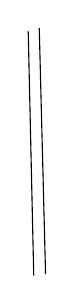
\begin{tikzpicture}[x=1cm,y=1cm]
\draw (0,0) -- (0.07,-3.1);
\draw (0.14,0.04) -- (0.22,-3.08);
\end{tikzpicture}}}
Je vais définir une équivalence de catégories
\diagram{\begin{tikzcd}[column sep=large,row sep=large]
{\text{(79)}\quad\uline{\unsure{\mathrm{Germarc\,diff}|\mathrm{Courarc\,diff}}}(X,x)} \arrow[r,"\approx"] \arrow[d,"\approx"{rotate=90}] &
\Pi_1(\mathbb S_x) \arrow[d,"\approx"{rotate=90}]\\
\uline{\mathrm{Rev\,uni}}(D_x^*) & \uline{\mathrm{Rev\,uni}}(\mathbb S_x)
\end{tikzcd}}
qui, sur les ensembles d'objets, soit l'application \unsure{associant} à $\forall$ germe d'arc différentiable en $x$ sa demi-\uline{tangente}. Il s'agit donc, si $\gamma,\gamma'$ sont deux tels arcs, correspondant à des demi-tangentes $\Delta,\Delta'$, de définir une bijection canonique


\scanpage{256}

\margin{\figure{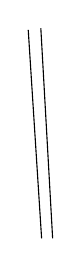
\begin{tikzpicture}[x=1cm,y=1cm]
\draw (0,0) -- (0.17,-2.65);
\draw (0.16,0.02) -- (0.31,-2.65);
\end{tikzpicture}}}
\diagram{\begin{tikzcd}[column sep=huge,row sep=large]
{\text{(80)}\quad\mathrm{Isom}(\gamma,\gamma')} \arrow[r,"\sim"] \arrow[d,equal,"\mathrm{d\acute ef}"] &
\mathrm{Isom}_{\Pi_1\mathbb S_x}(\Delta,\Delta') \arrow[d,equal,"\mathrm{d\acute ef}"]\\
\mathrm{Isom}(D_{x,\gamma}^{*\sim},D_{x,\gamma'}^{*\sim}) &
{\begin{array}{l}
\text{classes de chemins}\\
\text{dans }\mathbb S_x^*\text{ de }\Delta\\
\text{à }\Delta'
\end{array}}
\end{tikzcd}}

\deleted{\illegible{1}}
Au lieu de définir directement la bijection (80), je vais définir plutôt un foncteur (qui sera une équivalence de catégories)
\diagram{\begin{tikzcd}[column sep=large]
{\text{(81)}\quad\Theta:\Pi_1(\mathbb S_x)} \arrow[r,"{(\deleted{\unsure{\to|\sim}}\approx)}"] &
\uline{\mathrm{Rev\,uni}}(D_x^*),
\end{tikzcd}}

Soit \deleted{$\mathcal A$}
\[
\tag{82}
\left\{
\begin{array}{l}
\mathcal A_x\text{ ens des parties }\inserted{\text{fermées}}\text{ }1\text{-connexes de }\mathbb S_x\\
(\text{i.e. des }\uline{\text{arcs}}\text{ de cercle dans }\mathbb S_x,\\
\quad\unsure{\text{pouvant}}\text{ être réduits }\unsure{\text{à}}\text{ des pts,}\\
\quad\text{mais }\ne\mathbb S_x)
\end{array}
\right.
\]
c'est un ensemble ordonné, \unsure{et on|donc} \deleted{l'ensemble} définit une catégorie ordonnée $\uline{\mathcal A}_x$ (les objets sont les $\in\mathcal A_x$, les flèches sont les inclusions) --- et on sait que le groupoïde enveloppant \inserted{$\uline{\mathrm{Gr}}(\uline{\mathcal A}_x)$} de cette catégorie ordonnée est canoniquement équivalent à $\Pi_1(\mathbb S_x)$,


\scanpage{257}
\mspage{776}

de façon précise, soit \deleted{$\unsure{\uline{\mathcal A}_{0x}|\uline{\mathcal A}_x}$}\inserted{$\uline{\mathrm{Gr}}_0(\uline{\mathcal A}_x)$} la sous-catégorie pleine de $\uline{\mathrm{Gr}}(\uline{\mathcal A}_x)$ (dont l'ens des objets est $\mathcal A_x$) dont les objets soient les arcs \uline{ponctuels}, \& on a alors une équivalence canonique
\diagram{\begin{tikzcd}[column sep=large]
{\text{(83)}\quad\uline{\mathrm{Gr}}_0(\uline{\mathcal A}_x)} \arrow[r,"\approx"] & \Pi_1(\mathbb S_x)
\end{tikzcd}}
qui sur les objets se réduit à $\{a\}\longmapsto a$, et qui, pour tout arc \deleted{$\unsure{\mathbb S|\xi}$} $A$ d'extrémités $a,b$, d'où des isom d'inclusion \unsure{ds|dans} $\uline{\mathrm{Gr}}(\mathcal A_x)$
\diagram{\begin{tikzcd}[column sep=normal,row sep=large]
{\text{(84)}\quad\raisebox{-1.6em}{$\left\{\rule{0pt}{3.2em}\right.$}} &
a \arrow[r,"\sim"] & A & b \arrow[l,"\sim"'] & \\
& \text{d'où}\quad a \arrow[rr,"\sim"] & & b & \text{dans }\uline{\mathrm{Gr}}(\mathcal A_x)
\end{tikzcd}}
associe à cette flèche $a\overset{\sim}{\longrightarrow}b$ de $\uline{\mathrm{Gr}}_0(\mathcal A_x)$ la flèche de $\Pi_1(\mathbb S_x)$, définie par l'arc $A$ considéré comme chemin de $a$ en $b$.

Ainsi, pour $\forall$ groupoïde $\mathcal G$, la donnée d'un foncteur
\diagram{\begin{tikzcd}[column sep=large]
{\text{(85)}\quad\Psi:\Pi_1(\mathbb S_x)} \arrow[r] & \mathcal G
\end{tikzcd}}
équivaut à la donnée d'un foncteur

\scanpage{258}
\[
\tag{86}
\Psi : \underline{\mathcal A}_x \longrightarrow \mathcal G
\]
et (85) est une équivalence de cat. ssi
$\mathcal G$ est \deleted{\unsure{connexe}} connexe et
\deleted{\unsure{le}} son $\unsure{\pi_1|\Pi_1}$ est $\simeq\mathbb Z$, et si, pour
\deleted{\unsure{un $x$ de}}\inserted{un couple $(a,b)$ de}
pts $a,b$ distincts de $\unsure{\mathbb S_x}$, définissant deux arcs $A$ et $B$
d'extrémités $a,b$, \deleted{de}considérant l'autom de $a$ dans
$\underline{\mathrm{Gr}}_0(\mathcal A_x)$ i.e. dans
$\underline{\mathrm{Gr}}(\mathcal A_x)$, composé de
\[
\tag{86bis}
\diagram{\begin{tikzcd}[column sep=small]
\{a\} \arrow[r,"\sim"] & A & \{b\} \arrow[l,"\sim"'] \arrow[r,"\sim"] & B & \{a\} \arrow[l,"\sim"']
\end{tikzcd}}
\]
l'autom correspondant de $\Psi(\{a\})$ dans $\mathcal G$
soit un \uline{générateur} de $\mathrm{Aut}_{\mathcal G}(\Psi(\{a\}))$.

Nous allons donc définir un foncteur
\[
\tag{87}
\underline{\mathcal A}_x \longrightarrow
\underline{\mathrm{Revuni}}(D_x^*)
\]
\deleted{et} (satisfaisant la condition supplémentaire énoncée).
Pour définir un tel foncteur, il suffit de définir un foncteur
\[
\tag{88}
\underline{\mathcal A}_x \longrightarrow
\begin{gathered}
\text{catégorie des germes 1-connexes}\\
\text{d'espaces, \unsure{au|en} dessus du}\\
\text{germe }D_x^*
\end{gathered}
\]

\scanpage{259}
\mspage{777}
en composant ce foncteur avec le foncteur
\[
\tag{89}
\begin{gathered}
\text{cat. des germes 1-conn.}\\
\text{d'espaces \unsure{au|en} dessus}\\
\text{du germe }D_x^*
\end{gathered}
\longrightarrow \underline{\mathrm{Revuni}}(D_x^*).
\]
En fait, (88) \unsure{va associer|on associe} à $\forall\ A\in
\deleted{\unsure{\mathcal E}}\mathcal A_x$ un
\deleted{germe de \unsure{sous-espace} de $X$ en $x$, dont}
\inserted{filtre sur $X-x$ tendant vers $x$, dont}
on prendra le germe \deleted{\unsure{résiduel}}.

\deleted{\unsure{Les demi-droites}}
\inserted{Les éléments \inserted{$A$} de}
$\mathcal A_x$ s'identifient évidemment aux \uline{cônes}
\deleted{\unsure{ouverts}}\inserted{fermés $C$}
dans $\mathrm{Tang}_x(X)$, \deleted{\unsure{disti}}
distincts de $\{0\}$ et de l'espace
\inserted{\unsure{tang$^{\mathrm t}$|tangent}} $\forall$ entier.
\deleted{\unsure{Soit $C$ un}}
\inserted{Soit $\unsure{C\mathcal A_x|C\in\mathcal C\mathcal A_x}$ l'un de ces cônes.}
Considérons un isom local
\deleted{\unsure{un}}
\[
\tag{90}
f:(\mathrm{Tang}_x(X),0)\deleted{\unsure{\&}}
\xrightarrow{\sim}(X,x),
\]
\deleted{dont l'appl.}
\inserted{dont l'appl.} tangente soit l'identité.
\deleted{Lorsque} Si $C$ est un cône $\in\mathcal C\mathcal A_x$,
son image par un tel isom. dépend du choix de l'iso. local envisagé.
Mais considérons la \deleted{\unsure{famille|ensemble des}}
\inserted{base de filtre}
\deleted{\unsure{arcs}}\inserted{des} cônes
\inserted{$C'\in\mathcal C\mathcal A_x$} contenant
\deleted{$\unsure{\in}$} $C$ \uline{strictement}
(i.e. correspondant à des arcs $A'$ qui soient des \uline{voisinages}
de $A$, ou encore tels que $C'-\{0\}$ soit un voisinage de
$C\setminus\{0\}$), alors le

\scanpage{260}
\deleted{germe d'espace défini par la base}
\inserted{l'image par (90) \deleted{\unsure{de cette}}
\inserted{du filtre défini par la} base de}
filtre sur $\mathrm{Tang}_x(X)$ formé des
$V\cap(C'\setminus\{0\})$ \unsure{, où|:} $V$
parcourant les voisinages de $0$ dans $\mathrm{Tang}_x(X)$,
est un filtre sur $X\setminus\{x\}$ qui ne dépend plus du choix de $f$,
et qui tend vers $x$, donc définit un germe d'espace
\inserted{$\widetilde A$ ou $\widetilde C$}
au dessus de \deleted{$\unsure{X_x|X}$} $D_x^*$.
Ce germe d'espace, \deleted{\unsure{est é|et il}}
isom. au germe d'espace défini par $\mathrm{Tang}_x(X)$ muni du filtre
de base les $V\cap(C'-\{0\})$ --- où on peut prendre des $V$
convexes fermés \unsure{simétriques|symétriques}, donc
$V\cap(C'-\{0\})$ contractibles --- est évidemment 1-connexe.
Pour $A$ i.e. $C$ variable \unsure{i.e.} pour $A_1\subset A_2$
i.e. $C_1\subset C_2$ on a la relation correspondante d'inclusion
\inserted{\deleted{$\unsure{A}$}
\diagram{\begin{tikzcd}
\widetilde C_1 \arrow[r] & \widetilde C_2
\end{tikzcd}}}
sur les germes d'espaces dans $D_x^*$.
On trouve donc bien (88), d'où (87)\inserted{et (81)}, et on vérifie
que ce dernier est bien une équivalence de \deleted{catégories}
groupoïdes, via la \unsure{vérification|vérific$^{\mathrm t}$}
\deleted{\unsure{par}} \unsure{explicitée|explicité} plus haut ((86bis)).

\scanpage{261}
\mspage{778}
Considérons maintenant, à nouveau, un arc différentiable $\gamma$ dans $X$
sortant de $x$, et sa demi-tangente $\Delta$.
Alors $\{\Delta\}\in\mathcal A_x$, et on peut considérer le germe
d'espace $\{\Delta\}^{\sim}$ au dessus de $D_x^*$.
On a \inserted{\unsure{les|des}} deux morphismes d'inclusion canoniques
\[
\tag{91}
\diagram{\begin{tikzcd}
\gamma \arrow[r,hook] & \{\Delta\}^{\sim} \arrow[r,hook] & D_x^*
\end{tikzcd}}
\]
et on en déduit un isom. canonique
\[
\tag{92}
\diagram{\begin{tikzcd}[column sep=large]
\mathrm{Revuni}(D_x^*,\gamma) \arrow[r,phantom,"\simeq"] \arrow[d,equal,"\mathrm{déf}"]
& \mathrm{Revuni}(D_x^*,\{\Delta\}^{\sim}) \arrow[d,equal,"\mathrm{déf}"] \\
D_{x,\gamma}^{*\sim} & \Theta(\Delta)
\end{tikzcd}}
\]
Si $\gamma'$ est un autre arc diff. en $x$, correspondant à la demi-tangente
$\Delta'$, on a donc
\[
D_{x,\gamma}^{*\sim}\simeq\Theta(\Delta),\qquad
D_{x,\gamma'}^{*\sim}=\Theta(\Delta')
\]
d'où
\[
\diagram{\begin{tikzcd}[column sep=large,row sep=large]
\mathrm{Isom}(D_{x,\gamma}^{\unsure{*}\sim}\unsure{\}},D_{x,\gamma'}^{*\sim})
\arrow[r,phantom,"\simeq"] \arrow[d,equal,"\mathrm{déf}"]
& \mathrm{Isom}(\Theta(\Delta),\Theta(\Delta')) \\
\mathrm{Isom}(\gamma,\gamma')
& \mathrm{Isom}_{\Pi_1(\mathbb S_x)}(\Delta,\Delta')
\arrow[u,"\sim","\Theta"']
\end{tikzcd}}
\]
ce qui est la \deleted{\unsure{bonne}} bijection (80) cherchée.

\deleted{Soit} En résumé, on a un diagramme ess. comm. d'équivalences
de groupoïdes

\scanpage{262}
\[
\tag{93}
\diagram{\begin{tikzcd}[column sep=huge,row sep=huge]
\underline{\mathrm{germesdiff}}(X,x)
\arrow[r,"{\substack{\gamma\longrightarrow\underline\Delta(\gamma)\\\approx}}"]
\arrow[d,"\approx","{\substack{\gamma\mapsto\mathrm{Revuni}(D_x^*,\gamma)\\=D_{x,\gamma}^{*\sim}}}"']
& \Pi_1(\mathbb S_x)
\arrow[d,"{\approx\quad a\mapsto\mathrm{Revuni}(\mathbb S_x,\cdot)}"]
\arrow[dl,dashed,"{\Theta\ \approx}"'] \\
\underline{\mathrm{Rev.uni.}}(D_x^*) \arrow[r,"\approx"]
& \mathrm{Revuni.}(\mathbb S_x)
\end{tikzcd}}
\]
\margin{Bien sûr, la difficulté ici provenait du fait qu'on n'avait pas
de morphisme direct entre le germe $D_x^*$, et l'espace $\mathbb S_x$...}

\unsure{Le} seul foncteur qui n'ait pas encore explicité est le foncteur
\[
\tag{94}
\diagram{\begin{tikzcd}[column sep=small,row sep=small]
\underline{\mathrm{Revuni}}(D_x^*)
\arrow[rr,"\approx"] \arrow[dr,dashed,"{\Theta^{-1}}"']
& & \mathrm{Revuni}(\mathbb S_x) \\
& \Pi_1(\mathbb S_x) \arrow[ur,"{\mathrm{can}}"'] &
\end{tikzcd}}
\]
défini comme composé de $\Theta^{-1}$ avec le foncteur can.
$\Pi_1(\mathbb S_x)\longrightarrow\mathrm{Rev.uni.}(\mathbb S_x)$.

Finalement, dans ces considérations de géométrie topologique différentielle,
la construction-clef est celle du foncteur $\Theta$ (81).
Nous avons pris quelque peine à le définir de façon invariante.
Dans le cas où on dispose d'un iso local
\[
\tag{90}
f:\bigl(\underbrace{\mathrm{Tang}_x(X)}_{V},0\bigr)\longrightarrow(X,x),
\]
la construction de \unsure{ce|---} $\Theta$ peut s'expliciter comme
une construction canonique dans un espace vectoriel $V$.
Toute demi-droite hom.

\scanpage{263}
\mspage{779}

$\Delta$ dans $V$ définit un germe d'arc (\unsure{diff.}) dans $V$ sortant de $0$, d'où un rev. universel correspondant $D_{V,0;\Delta}^{*\sim}$ de $D_{V,0}^{*}$, donc un rev. universel $D_{x,\Delta}^{*\sim}$ de $D_x^*$.
Il faut voir comment ce $D_{x,\Delta}^{*\sim}$ dépend ``continûment'' de $\Delta$, et ce qui revient au $\overline{\mathrm m}$, comment le rev. universel $V_{\Delta}^{*\sim}$ de $V^*=V\setminus\{0\}$ dépend continûment de $\Delta$, ce qui est tout à fait \unsure{standard}\unsure{...}.

Soit maintenant \inserted{$\unsure{u|\varphi}$} \unsure{un} un \deleted{difféomorphisme}\inserted{\unsure{automorphisme}} de $X$, fixant $x$, et différentiable en $x$. On a donc \deleted{\unsure{des}} \unsure{autom.} induits \deleted{de}
\[
\tag{\unsure{95|94}}
{}^{\unsure{u|\varphi}}D_x^*\quad\text{autom. de }D_x^*,\qquad
{}^{\unsure{u|\varphi}}\mathbb S_x\quad\text{autom. de }\mathbb S_x.
\]

Considérons d'autre part un rev. universel $\widetilde{\mathbb S}_x$ de $\mathbb S_x$, et soit $D_x^{*\sim}$ un rev. universel de $D_x^*$ associé, grâce à l'équiv. (94). Je dis qu'on a alors une

\scanpage{264}

bijection canonique
\[
\tag{96}
\diagram{\begin{array}{c@{\qquad}c@{\qquad}c}
\text{ens des relèvements}&\simeq&\text{ens des relèvements}\\
\text{de }{}^uD_x^*\text{ en un}&&\text{de }{}^u\mathbb S_x\text{ en un}\\
\text{autom }{}^uD_x^{*\sim}\text{ du}&&\text{autom }{}^u\mathbb S_x^\sim\text{ de}\\
\text{germe }D_x^{*\sim}&&\mathbb S_x^\sim
\end{array}},
\]
\margin{la construction (96) sera faite dans les pages qui suivent, aboutissant à (122) p.\unsure{783}}
bijection qui soit un isomorphisme de $\overline T_x$-torseurs.
(où $\overline T_x$ est le $\mathbb Z$-module d'orientation de $X$ en $x$, rappelons-le).

\margin{E) \uline{Axiomatisation} : \unsure{la structure|structure} de \uline{corrélation} entre rev. universels $\mathbb S_x^\sim$ \uline{et} $D_x^{*\sim}$.}
J'ai envie de donner une description axiomatique de (94) et (96).

1) Soit \inserted{$D_x=$} $(X,x)$ un germe de surface différentiable, d'où
$V_{X,x}=V_x=\mathbb V=\operatorname{Tang}_x(X)$,
et $\mathbb S_x=V^*/\mathbb R^{*+}$ (où $\mathbb V^*=V\setminus\{0\}$), ainsi que $D_{X,x}^*=D_x^*$.
\margin{``germe'' : on \unsure{sous-entend} le filtre des voisinages de $x$ dans $X$}
\deleted{Soit $\mathbb S_x^\sim$ (\unsure{resp.} $D_x^{*\sim}$) des rev. \unsure{universels} de $\mathbb S_x$ (resp. $D_x^*$).}
\inserted{On désigne par}
\deleted{$\unsure{\mathcal A|\in}$}
$\mathcal A_{X,x}$ \unsure{ou} $\mathcal A_x$ l'ens des \uline{arcs} de $\mathbb S_x$, en corr. biunivoque avec l'ens $\mathcal C_{X,x}=\mathcal C_x$ des
\deleted{``\unsure{secteurs angulaires}'' de $V$ \unsure{propres}}
\inserted{``cônes fermés'' \unsure{propres}} de $V$ ($\ne V$ et $\{0\}$).
Pour $A\in\mathcal A_x$ ou $C\in\mathcal C_x$, on désigne par
\deleted{$\unsure{\widetilde A|f(A)}$ \unsure{ou} $\unsure{\widetilde C|f(C)}$}
\inserted{$\unsure{\mathrm{Ep}|E_p}(A)$ ou $\unsure{\mathrm{Ep}|E_p}(C)$}
le germe d'espace correspondant au-dessus de $D_x^*$.
\margin{``\unsure{épaississement}'' \deleted{\unsure{image|germe}} de $A$ (ou de $C$) dans $D_x^*$}
Si $\widetilde{\mathbb S}$ est un rev. uni. de $\mathbb S$, $\widetilde D_x^*$ un rev. universel de $\widetilde D_x^*$, on considère les ens

\scanpage{265}
\mspage{780}

\[
\tag{97}
\diagram{\begin{array}{r@{\,}c@{\qquad}c@{\qquad}r@{\,}c}
&\Gamma\bigl(\deleted{\unsure{\mathbb S|\widetilde A}}A,\mathbb S_x^\sim/\mathbb S_x\bigr)&,&
&\Gamma\bigl(\inserted{\unsure{\mathrm{Ep}|E_p}}(\widetilde A),D_x^{*\sim}/D_x^*\bigr)\\
&\Vert&&&\Vert\\
&\operatorname{Hom}_{\mathbb S}(A,\mathbb S_x^\sim)&&&\operatorname{Hom}_{D_x^*}(\widetilde A,D_x^{*\sim})\\
\mathrm{déf}&\Vert&&\mathrm{déf}&\Vert\\
&\mathbb S_x^\sim(A)&&&D_x^{*\sim}\bigl(\unsure{\mathrm{Ep}|E_p}(A)\bigr)
\end{array}}
\]
qui sont l'un et l'autre Torseurs sur le $\overline{\mathrm m}$ groupe $\overline T_{X,x}=\overline T_x$ (le $\mathbb Z$-module des orientations de $X$ au point $x$). Considérons l'ens
\[
\tag{98}
H(A)=\operatorname{Isom}_{\unsure{T_x|\overline T_x}}\bigl(\mathbb S_x^\sim(A),
\deleted{\unsure{D_x^{*\sim}(\widetilde A)}}\unsure{)}
\inserted{D_x^{*\sim}\bigl(\unsure{\mathrm{Ep}|E_p}(A)\bigr)}\bigr)
\]
qui est lui-$\overline{\mathrm m}$ un $\overline T_x$-torseur. Si on a \deleted{\illegible{1}} une inclusion
\[
A\subset A'
\]
on en déduit, par restriction, des isom. de $\overline T_x$-torseurs
\[
\tag{99}
\mathbb S_x^\sim(A')\xrightarrow{\sim}\mathbb S_x^\sim(A),\qquad
D_x^{*\sim}\bigl(\unsure{\mathrm{Ep}|E_p}(A')\bigr)
\unsure{-|\longrightarrow}
D_x^{*\sim}\bigl(\unsure{\mathrm{Ep}|E_p}(A)\bigr)
\]
d'où un isom. canonique
\[
\tag{100} H(A)\xrightarrow{\sim}H(A')
\]
de sorte que \deleted{$A\unsure{\longmapsto|\longleftarrow}H(A)$ \unsure{définit}}
\[
\tag{101}
A\longmapsto H(A),\quad\text{foncteur}\quad
\underline{\mathcal A}_x\xrightarrow{H}\underline{\operatorname{Tors}}(\overline T_x),
\]
où $\underline{\mathcal A}_x$ est la catégorie ordonnée associée à l'ens ordonné $\mathcal A_x$. On trouve donc par factorisation un foncteur \unsure{du|de} \deleted{la catégorie} groupoïde enveloppant de $\underline{\mathcal A}_x$ dans $\underline{\operatorname{Tors}}(\overline T_x)$;
\[
\tag{102}
\diagram{\begin{tikzcd}[column sep=large,row sep=large]
&\underline{\mathcal A}_x\arrow[dl,"{\unsure{\rho|\gamma}}"']\arrow[dr,"H"]&\\
\underline{\operatorname{Gr}}(\underline{\mathcal A}_x)\arrow[rr,"{\underline{\operatorname{Gr}}(H)}"]&&\underline{\operatorname{Tors}}(\overline T_x)
\end{tikzcd}}.
\]

\scanpage{266}

\deleted{Je dis que}\inserted{On sait que} $\underline{\operatorname{Gr}}(\underline{\mathcal A}_x)$ est \deleted{\unsure{isomorphe}} un $\overline T_x$-groupoïde, de façon précise le foncteur
\[
\deleted{\operatorname{Hom}_{\underline{\operatorname{Gr}}(\underline{\mathcal A}_x)}(A,A')\xrightarrow{\sim}}
\]
\[
\tag{103}
\diagram{$\left\{\begin{array}{rcl}
\underline{\mathcal A}_x&\longrightarrow&\underline{\operatorname{Revuni}}(\mathbb S_x)\overset{\mathrm{déf}}{=}\mathbb S_{x,A}^{\deleted{\unsure{*}}\sim}\\[1ex]
A&\longmapsto&\deleted{\unsure{\mathbb S}}\operatorname{Revuni}(\mathbb S,A)
\end{array}\right.$}
\]
qui se factorise en un \deleted{foncteur}\inserted{morphisme} de groupoïdes
\[
\tag{104}
\underline{\operatorname{Gr}}(\underline{\mathcal A}_x)\xrightarrow{(\simeq)}\underline{\operatorname{Rev.uni.}}(\mathbb S_x)
\]
donne une \uline{équivalence de cat.} (104), donc
\[
\tag{105}
\operatorname{Hom}_{\underline{\operatorname{Gr}}(\underline{\mathcal A}_x)}(A,A')\xrightarrow{\sim}
\operatorname{Hom}_{\deleted{\unsure{\underline{\operatorname{Revuni}}}}\inserted{\unsure{\mathbb S_x}}}(\mathbb S_{x,A}^{\sim},\mathbb S_{x,A'}^{\sim})
\]
\margin{\unsure{i.e. on a pour} $A,A'\in\mathcal A_x$, \unsure{l'iso. can}
\[
\operatorname{Hom}_{\underline{\operatorname{Gr}}(\underline{\mathcal A}_x)}(A,A')\simeq
\operatorname{Isom}_{\underline{\operatorname{Revuni}}(\mathbb S_x)}(\mathbb S_{x,A}^{\sim},\mathbb S_{x,A'}^{\sim}).
\]}

Ceci \deleted{\unsure{fait|étant}} rappelé, je dis que le foncteur $\underline{\operatorname{Gr}}(H)$ de (102) est \uline{essentiellement} \unsure{constant} \inserted{i.e. il définit sur les $\pi_1$ l'hom. nul $\overline T_x\xrightarrow{0}\overline T_x$} --- ou ce qui revient au $\overline{\mathrm m}$, il y a entre les $H(A)$, \inserted{en comprenant les isom (100),} un \uline{système transitif} d'\uline{isomorphismes}. On désigne alors \deleted{par} la ``valeur commune'' de ces $H(A)$, qui ne dépend que du choix de $\mathbb S_x^{\sim}$ et de $D_x^{*\sim}$, par $H(\mathbb S_x^{\sim},D_x^{*\sim})$. \deleted{\unsure{On a donc}}\inserted{Cet ens} est muni de la structure définie par des isom de $\overline T_x$-\unsure{torseurs|foncteurs}
\[
\tag{106}
\unsure{i_A|\widetilde{\imath}_A}:H(A)\xrightarrow{\sim}H(\mathbb S_x^{\sim},D_x^{*\sim})
\]
satisfaisant la condition de compatibilité, s'expri-
